\documentclass[tikz,border=20pt]{standalone}
\usepackage{tikz}
\usetikzlibrary{arrows.meta,calc}

\begin{document}

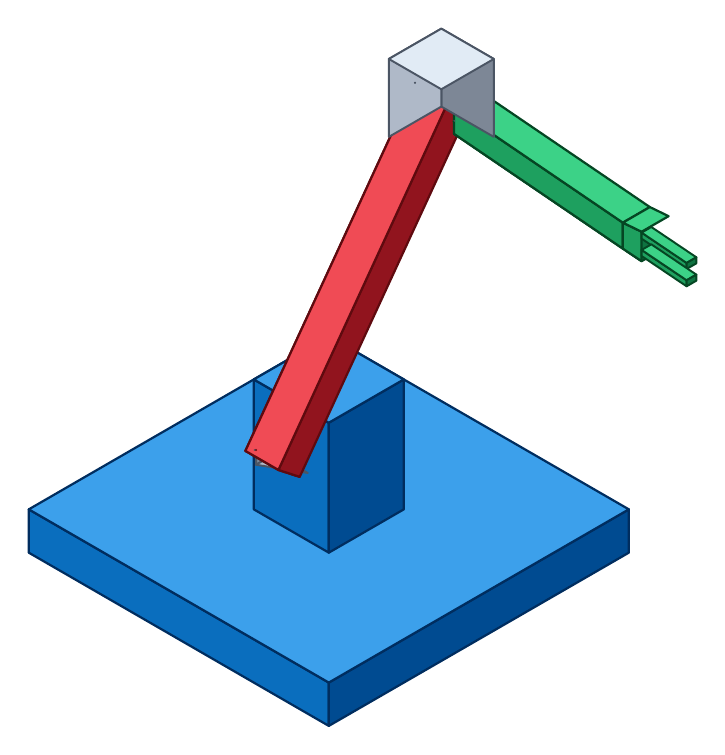
\begin{tikzpicture}[
    x={(-0.866cm,-0.5cm)}, 
    y={(0.866cm,-0.5cm)}, 
    z={(0cm,1.0cm)},
    scale=1.1, 
    line cap=round, 
    line join=round
]

    % ==========================================
    % CAD COLOR PALETTE (Realistic Technical CAD Shading)
    % ==========================================
    \definecolor{cadBlueTop}{RGB}{60, 160, 235}
    \definecolor{cadBlueLeft}{RGB}{10, 110, 190}
    \definecolor{cadBlueRight}{RGB}{0, 75, 145}
    \definecolor{cadBlueLine}{RGB}{0, 45, 95}

    \definecolor{cadRedTop}{RGB}{240, 75, 85}
    \definecolor{cadRedLeft}{RGB}{195, 35, 45}
    \definecolor{cadRedRight}{RGB}{145, 20, 30}
    \definecolor{cadRedLine}{RGB}{95, 10, 15}

    \definecolor{cadGreenTop}{RGB}{60, 210, 135}
    \definecolor{cadGreenLeft}{RGB}{30, 160, 95}
    \definecolor{cadGreenRight}{RGB}{15, 115, 65}
    \definecolor{cadGreenLine}{RGB}{5, 70, 35}

    \definecolor{cadMetalTop}{RGB}{225, 235, 245}
    \definecolor{cadMetalLeft}{RGB}{175, 185, 200}
    \definecolor{cadMetalRight}{RGB}{125, 135, 150}
    \definecolor{cadMetalLine}{RGB}{75, 85, 100}

    % ==========================================
    % 1. BASE PLATE (Solid Blue Cuboid)
    % Bounds: X: [-2.0, 2.0], Y: [-2.0, 2.0], Z: [-0.5, 0]
    % ==========================================
    
    % Front-Left Face (X = 2.0)
    \draw[fill=cadBlueLeft, draw=cadBlueLine, line width=0.8pt]
        (2.0, -2.0, -0.5) -- (2.0, 2.0, -0.5) -- (2.0, 2.0, 0) -- (2.0, -2.0, 0) -- cycle;

    % Front-Right Face (Y = 2.0)
    \draw[fill=cadBlueRight, draw=cadBlueLine, line width=0.8pt]
        (-2.0, 2.0, -0.5) -- (2.0, 2.0, -0.5) -- (2.0, 2.0, 0) -- (-2.0, 2.0, 0) -- cycle;

    % Top Face (Z = 0)
    \draw[fill=cadBlueTop, draw=cadBlueLine, line width=0.8pt]
        (-2.0, -2.0, 0) -- (2.0, -2.0, 0) -- (2.0, 2.0, 0) -- (-2.0, 2.0, 0) -- cycle;


    % ==========================================
    % 2. VERTICAL TOWER BLOCK (Solid Blue Cuboid)
    % Bounds: X: [-0.5, 0.5], Y: [-0.5, 0.5], Z: [0, 1.5]
    % ==========================================

    % Front-Left Face (X = 0.5)
    \draw[fill=cadBlueLeft, draw=cadBlueLine, line width=0.8pt]
        (0.5, -0.5, 0) -- (0.5, 0.5, 0) -- (0.5, 0.5, 1.5) -- (0.5, -0.5, 1.5) -- cycle;

    % Front-Right Face (Y = 0.5)
    \draw[fill=cadBlueRight, draw=cadBlueLine, line width=0.8pt]
        (-0.5, 0.5, 0) -- (0.5, 0.5, 0) -- (0.5, 0.5, 1.5) -- (-0.5, 0.5, 1.5) -- cycle;

    % Top Face (Z = 1.5)
    \draw[fill=cadBlueTop, draw=cadBlueLine, line width=0.8pt]
        (-0.5, -0.5, 1.5) -- (0.5, -0.5, 1.5) -- (0.5, 0.5, 1.5) -- (-0.5, 0.5, 1.5) -- cycle;


    % ==========================================
    % 3. SHOULDER JOINT 1 (Pivot Shaft)
    % ==========================================
    \draw[fill=cadMetalRight, draw=cadMetalLine, line width=0.7pt]
        (0.5, -0.22, 0.78) -- (0.75, -0.22, 0.78) -- (0.75, -0.22, 1.22) -- (0.5, -0.22, 1.22) -- cycle;

    \draw[fill=cadMetalLeft, draw=cadMetalLine, line width=0.7pt]
        (0.5, -0.22, 0.78) -- (0.75, -0.22, 0.78) -- (0.5, 0.22, 0.78) -- (0.5, 0.22, 0.78) -- cycle;


    % ==========================================
    % 4. LINK 1 (Zusammenhängender Roter Quader)
    % Solid beam extending from Joint 1 (0.75, 0, 1.0) to Joint 2 (-1.5, 0, 4.0)
    % ==========================================

    % Bottom End Plate (closing the J1 bottom of red beam)
    \draw[fill=cadRedLeft, draw=cadRedLine, line width=0.8pt]
        (0.608, -0.22, 0.789) -- (0.608, 0.22, 0.789) -- (0.892, 0.22, 1.011) -- (0.892, -0.22, 1.011) -- cycle;

    % Front-Right Face (Y = +0.22)
    \draw[fill=cadRedRight, draw=cadRedLine, line width=0.8pt]
        (0.608, 0.22, 0.789) -- (-1.642, 0.22, 3.889) -- (-1.358, 0.22, 4.111) -- (0.892, 0.22, 1.011) -- cycle;

    % Front-Left Face (Y = -0.22)
    \draw[fill=cadRedLeft, draw=cadRedLine, line width=0.8pt]
        (0.608, -0.22, 0.789) -- (-1.642, -0.22, 3.889) -- (-1.358, -0.22, 4.111) -- (0.892, -0.22, 1.011) -- cycle;

    % Top Face (Upper Surface)
    \draw[fill=cadRedTop, draw=cadRedLine, line width=0.8pt]
        (0.892, -0.22, 1.011) -- (-1.358, -0.22, 4.111) -- (-1.358, 0.22, 4.111) -- (0.892, 0.22, 1.011) -- cycle;

    % Joint 1 Cylindrical Cap (Schultergelenk-Nabe)
    \draw[fill=cadRedLeft, draw=cadRedLine, line width=0.8pt]
        (0.75, -0.22, 0.95) circle [x={(0,0.34cm)}, y={(0,0,0.34cm)}];
    \draw[fill=cadMetalTop, draw=cadMetalLine, line width=0.6pt]
        (0.76, -0.23, 0.95) circle [x={(0,0.17cm)}, y={(0,0,0.17cm)}];


    % ==========================================
    % 5. LINK 2 (Zusammenhängender Grüner Quader)
    % ==========================================

    % Top Cap at J2 for Link 1 (Closing top of red beam)
    \draw[fill=cadRedTop, draw=cadRedLine, line width=0.8pt]
        (-1.642, -0.22, 3.889) -- (-1.642, 0.22, 3.889) -- (-1.358, 0.22, 4.111) -- (-1.358, -0.22, 4.111) -- cycle;

    % Green Beam Body
    % Front-Right Face (Y-side)
    \draw[fill=cadGreenRight, draw=cadGreenLine, line width=0.8pt]
        (-1.68, 0.35, 3.85) -- (-1.68, 2.60, 3.65) -- (-1.32, 2.60, 3.65) -- (-1.32, 0.35, 3.85) -- cycle;

    % Front-Left Face (X = -1.32)
    \draw[fill=cadGreenLeft, draw=cadGreenLine, line width=0.8pt]
        (-1.32, 0.35, 3.85) -- (-1.32, 2.60, 3.65) -- (-1.32, 2.60, 3.95) -- (-1.32, 0.35, 4.15) -- cycle;

    % Top Face (Z-upper)
    \draw[fill=cadGreenTop, draw=cadGreenLine, line width=0.8pt]
        (-1.68, 0.35, 4.15) -- (-1.68, 2.60, 3.95) -- (-1.32, 2.60, 3.95) -- (-1.32, 0.35, 4.15) -- cycle;

    % Joint 2 Ellbogengelenk-Nabe (Verbindung zwischen Arm 1 und Arm 2)
    \draw[fill=cadMetalLeft, draw=cadMetalLine, line width=0.8pt]
        (-1.32, 0.35, 4.0) circle [x={(0,0.34cm)}, y={(0,0,0.34cm)}];
    \draw[fill=cadGreenTop, draw=cadGreenLine, line width=0.6pt]
        (-1.31, 0.35, 4.0) circle [x={(0,0.17cm)}, y={(0,0,0.17cm)}];


    % ==========================================
    % 6. END EFFECTOR / GREIFER (CAD Tool Head)
    % ==========================================

    % Tool Base Mount Block (Green Solid Cuboid)
    \draw[fill=cadGreenRight, draw=cadGreenLine, line width=0.8pt]
        (-1.68, 2.60, 3.65) -- (-1.68, 2.85, 3.63) -- (-1.32, 2.85, 3.63) -- (-1.32, 2.60, 3.65) -- cycle;

    \draw[fill=cadGreenLeft, draw=cadGreenLine, line width=0.8pt]
        (-1.32, 2.60, 3.65) -- (-1.32, 2.85, 3.63) -- (-1.32, 2.85, 3.97) -- (-1.32, 2.60, 3.95) -- cycle;

    \draw[fill=cadGreenTop, draw=cadGreenLine, line width=0.8pt]
        (-1.68, 2.60, 3.95) -- (-1.68, 2.85, 3.97) -- (-1.32, 2.85, 3.97) -- (-1.32, 2.60, 3.95) -- cycle;

    % Upper Claw Finger
    \draw[fill=cadGreenLeft, draw=cadGreenLine, line width=0.7pt]
        (-1.32, 2.85, 3.96) -- (-1.32, 3.45, 3.91) -- (-1.32, 3.45, 3.84) -- (-1.32, 2.85, 3.89) -- cycle;
    \draw[fill=cadGreenTop, draw=cadGreenLine, line width=0.7pt]
        (-1.45, 2.85, 3.96) -- (-1.45, 3.45, 3.91) -- (-1.32, 3.45, 3.91) -- (-1.32, 2.85, 3.96) -- cycle;
    \draw[fill=cadGreenRight, draw=cadGreenLine, line width=0.7pt]
        (-1.45, 3.45, 3.91) -- (-1.45, 3.45, 3.84) -- (-1.32, 3.45, 3.84) -- (-1.32, 3.45, 3.91) -- cycle;

    % Lower Claw Finger
    \draw[fill=cadGreenLeft, draw=cadGreenLine, line width=0.7pt]
        (-1.32, 2.85, 3.76) -- (-1.32, 3.45, 3.71) -- (-1.32, 3.45, 3.64) -- (-1.32, 2.85, 3.69) -- cycle;
    \draw[fill=cadGreenTop, draw=cadGreenLine, line width=0.7pt]
        (-1.45, 2.85, 3.76) -- (-1.45, 3.45, 3.71) -- (-1.32, 3.45, 3.71) -- (-1.32, 2.85, 3.76) -- cycle;
    \draw[fill=cadGreenRight, draw=cadGreenLine, line width=0.7pt]
        (-1.45, 3.45, 3.71) -- (-1.45, 3.45, 3.64) -- (-1.32, 3.45, 3.64) -- (-1.32, 3.45, 3.71) -- cycle;
    % Gelenk
    \draw[fill=cadMetalRight, draw=cadMetalLine, line width=0.7pt] 
        (-1.85, -0.35, 3.55) -- (-1.85, 0.35, 3.55) -- (-1.85, 0.35, 4.45) -- (-1.85, -0.35, 4.45) -- cycle; 
    \draw[fill=cadMetalLeft, draw=cadMetalLine, line width=0.7pt] 
        (-1.85, -0.35, 3.55) -- (-1.15, -0.35, 3.55) -- (-1.15, -0.35, 4.45) -- (-1.85, -0.35, 4.45) -- cycle; 
    % Frontal sichtbare kreisförmige Gelenkscheibe (Zylinder-Stirnfläche am Gelenk) 
    \draw[fill=cadMetalLeft, draw=cadMetalLine, line width=0.8pt] 
        (-1.50, -0.35, 4.00) circle [x={(0,0.55cm)}, y={(0,0,0.55cm)}]; 
    % Inlay / Prägung der Gelenk-Achse 
    \draw[fill=cadMetalTop, draw=cadMetalLine, line width=0.6pt] 
        (-1.50, -0.35, 4.00) circle [x={(0,0.38cm)}, y={(0,0,0.38cm)}]; 
    \draw[fill=cadMetalTop, draw=cadMetalLine, line width=0.5pt] 
        (-1.50, -0.35, 4.00) circle [x={(0,0.20cm)}, y={(0,0,0.20cm)}]; 
    % Oberer Zylinderdeckel (Aufsicht auf das Gelenk) 
    \draw[fill=cadMetalTop, draw=cadMetalLine, line width=0.7pt] 
        (-1.85, -0.35, 4.45) -- (-1.15, -0.35, 4.45) -- (-1.15, 0.35, 4.45) -- (-1.85, 0.35, 4.45) -- cycle;
\end{tikzpicture}
\end{document}
